
%----------------------------------------------------------------------------------------
%  Trapezoid rule with POSIX's Pthreads
%----------------------------------------------------------------------------------------

\section{Trapezoid rule with POSIX Pthreads}

\subsection{Creating threads using POSIX}

\vspace{0.5cm}
\lstinputlisting[
	style=CStyle,
	firstline=72, % First line of code
	lastline=75, % Lastl ine of code
	caption=Creating POSIX Pthreads (line 72-75 in lab2part2.c), % Caption above the listing
	label=lst:lab2part2a, % Label for referencing this listing
	frame=single, % Frame around the code listing
	showstringspaces=false, % Don't put marks in string spaces
	numbers=left, % Line numbers on left
	numberstyle=\normalsize % Line numbers styling
    ]{../code/lab2part2.c}

%----------------------------------------------------------------------------------------

\subsection{Joining threads using POSIX}

\vspace{0.5cm}
\lstinputlisting[
	style=CStyle,
	firstline=77, % First line of code
	lastline=80, % Lastl ine of code
	caption=Joining POSIX Pthreads (line 77-80 in lab2part2.c), % Caption above the listing
	label=lst:lab2part2b, % Label for referencing this listing
	frame=single, % Frame around the code listing
	showstringspaces=false, % Don't put marks in string spaces
	numbers=left, % Line numbers on left
	numberstyle=\normalsize % Line numbers styling
    ]{../code/lab2part2.c}

%----------------------------------------------------------------------------------------

\subsection{If each thread is allowed to increment the total sum on the fly, does a race condition exist?
If so, how does this affect the final result?}

With syncronisation, a race condition will exist when multiple thread increment the total sum at the same
time. This affects teh final result by making the global total sum to be less than the actual sum due
increments that were unaccounted for because they were done at the same time.

%----------------------------------------------------------------------------------------

\subsection{Mutex based critical section}

\vspace{0.5cm}
\lstinputlisting[
	style=CStyle,
	firstline=120, % First line of code
	lastline=122, % Lastl ine of code
	caption=Mutex based threads synchronisation (line 120-122 in lab2part2.c), % Caption above the listing
	label=lst:lab2part2c, % Label for referencing this listing
	frame=single, % Frame around the code listing
	showstringspaces=false, % Don't put marks in string spaces
	numbers=left, % Line numbers on left
	numberstyle=\normalsize % Line numbers styling
    ]{../code/lab2part2.c}

%----------------------------------------------------------------------------------------

\subsection{Semaphore based critical section}

\vspace{0.5cm}
\lstinputlisting[
	style=CStyle,
	firstline=110, % First line of code
	lastline=112, % Lastl ine of code
	caption=Semaphores based threads synchronisation (line 120-122 in lab2part2.c), % Caption above the listing
	label=lst:lab2part2d, % Label for referencing this listing
	frame=single, % Frame around the code listing
	showstringspaces=false, % Don't put marks in string spaces
	numbers=left, % Line numbers on left
	numberstyle=\normalsize % Line numbers styling
    ]{../code/lab2part2.c}

%----------------------------------------------------------------------------------------

\subsection{Busy-wait based critical section}

\vspace{0.5cm}
\lstinputlisting[
	style=CStyle,
	firstline=115, % First line of code
	lastline=117, % Lastl ine of code
	caption=Busy-wait based threads synchronisation (line 115-117 in lab2part2.c), % Caption above the listing
	label=lst:lab2part2e, % Label for referencing this listing
	frame=single, % Frame around the code listing
	showstringspaces=false, % Don't put marks in string spaces
	numbers=left, % Line numbers on left
	numberstyle=\normalsize % Line numbers styling
    ]{../code/lab2part2.c}

\subsection{Results}

The code was compile to compute the trapezoid rule for $a=0$, $b=1$, $n=2^{30}$ for the function $f(x)$.
128 threads were used for each of the three methods (mutex, semaphores, busy-wait) to determine whic method is the fastest.
The function $f(x)$ is hardwired to compute $x^2$, see \cref{lst:lab2part2f}.

\vspace{0.5cm}
\lstinputlisting[
	style=CStyle,
	firstline=154, % First line of code
	lastline=159, % Lastl ine of code
	caption=Hardwired f(x) for trapezoid rule (line 154-159 in lab2part2.c), % Caption above the listing
	label=lst:lab2part2f, % Label for referencing this listing
	frame=single, % Frame around the code listing
	showstringspaces=false, % Don't put marks in string spaces
	numbers=left, % Line numbers on left
	numberstyle=\normalsize % Line numbers styling
    ]{../code/lab2part2.c}

Linux echo was use to pipe in the user input so that it does not vary execution the execution time. Linux's
time command was used to time the different synchronisation methods. The results are shown in 
\cref{fig:part2_128_0,fig:part2_128_1,fig:part2_128_2}.

\begin{figure}[ht]
	\centering
	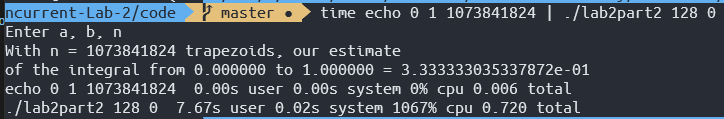
\includegraphics[width=\textwidth]{Figures/part2_128_1.PNG}
	\caption{Terminal output of lab2part2.c program using 128 threads and mutex}
	\label{fig:part2_128_0}
\end{figure}

\begin{figure}[ht]
	\centering
	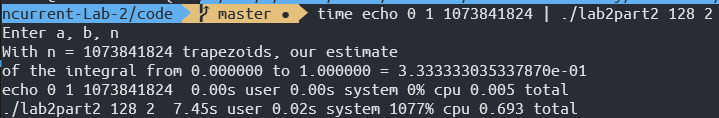
\includegraphics[width=\textwidth]{Figures/part2_128_2.PNG}
	\caption{Terminal output of lab2part2.c program using 128 threads and semaphores}
	\label{fig:part2_128_1}
\end{figure}

\begin{figure}[ht]
	\centering
	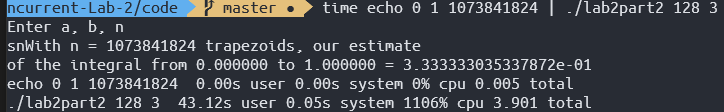
\includegraphics[width=\textwidth]{Figures/part2_128_3.PNG}
	\caption{Terminal output of lab2part2.c program using 128 threads and busy-wait}
	\label{fig:part2_128_2}
\end{figure}

The result shows that semaphores is the fastest, then mutex and then busy-wait in terms of execution time.
Busy wait is the least efficient because it consumes CPU cycles as the threads continously wait. Busy-wait
enfores the order of access to the critical section, and waits for the system to schedule on the thread
rank matching the flag variable to allow be allowed through - if it schedules on the wrong thread (a thread
that is busy-waiting), it wastes CPU cycles in the checking of the while condition until it deschedules and 
eventually until it picks the correct thread.

Mutex is middle between the three, only slower than semaphores by 40ms. The order the threads execute
the critical section is random, which does not guarentee that locks are given in the order they are called.